% Section 1 - The perception problem
% Roberto Masocco <roberto.masocco@uniroma2.it>
% June 5, 2024

% ### The perception problem ###
\section{The perception problem}
\graphicspath{{figs/section1/}}

% --- The perception problem ---
\begin{frame}{The perception problem}{Definition}
  To be able to operate autonomously, a robot must continuously answer the following questions:
  \begin{itemize}
    \item \textbg{Where am I?}
    \item \textbg{What is this place?}
  \end{itemize}
  \medskip
  Thus, it must be able to \textbg{perceive} the environment, gathering information useful to:
  \begin{itemize}
    \item \textbg{localize itself}, \emph{i.e.}, continuously estimate its \textbg{pose} as \textbg{both position and orientation} in 3D space;
    \item \textbg{map the environment}, \emph{i.e.}, build a \textbg{representation} of the environment useful to \textbg{navigate} within it.
  \end{itemize}
\end{frame}
\begin{frame}{The perception problem}{Challenges}
  The perception problem is challenging because:
  \begin{itemize}
    \item the environment may be \textbg{partially observable}, \emph{i.e.}, the robot can only perceive a \textbg{subset} of it, and need to update its information in real time;
    \item the environment may be \textbg{dynamic}, \emph{i.e.}, it can change over time;
    \item measurements are always subject to \textbg{noise}.
  \end{itemize}
  \medskip
  The perception problem is usually solved by \textbg{sensor fusion}, \emph{i.e.}, combining information from \textbg{multiple sensors} to obtain a more \textbg{accurate} and \textbg{reliable} estimate of the environment, possibly accounting for \textbg{sensor faults}.
\end{frame}
\begin{frame}{The perception problem}{Tools for the job}
  The tools that robots use to gather \textbg{measurements} from the environment are called \textbg{sensors}.\\
  \medskip
  They can be classified as:
  \begin{itemize}
    \item \textbg{proprioceptive}, \emph{i.e.}, measuring robotic interaction with the environment (\emph{e.g.}, \textbg{encoders}, \textbg{GPS}, \textbg{IMUs});
    \item \textbg{exteroceptive}, \emph{i.e.}, measuring the environment itself (\emph{e.g.}, \textbg{cameras}, \textbg{LiDARs}, \textbg{radars});
    \item \textbg{interoceptive}, \emph{i.e.}, measuring the robot's internal state.
  \end{itemize}
\end{frame}
\begin{frame}{The perception problem}{Tools for the job}
  As any other measurement tool, sensors are based on \textbg{physical principles} and \textbg{energy exchanges}, translating the information they gather into \textbg{electrical signals} that can be acquired and/or processed by a computer.\\
  \medskip
  They are usually characterized by at least:
  \begin{itemize}
    \item a \textbg{digital} or \textbg{analog} \textbg{encoding} of the measurement;
    \item a \textbg{frame of reference} in which the measurement is expressed;
    \item \textbg{accuracy} and \textbg{uncertainty} parameters.
  \end{itemize}
\end{frame}
\begin{frame}{The perception problem}{Tools for the job}
  \begin{figure}
    \centering
    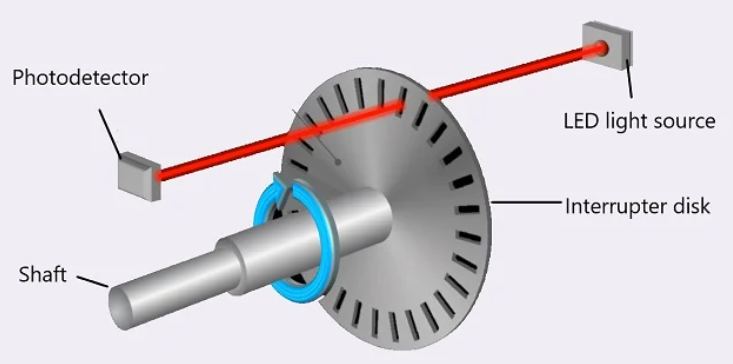
\includegraphics[width=.75\textwidth]{encoder.png}
    \caption{Rotary encoder working principle.}
    \label{fig:encoder}
  \end{figure}
\end{frame}
\begin{frame}{The perception problem}{Tools for the job}
  \begin{figure}
    \centering
    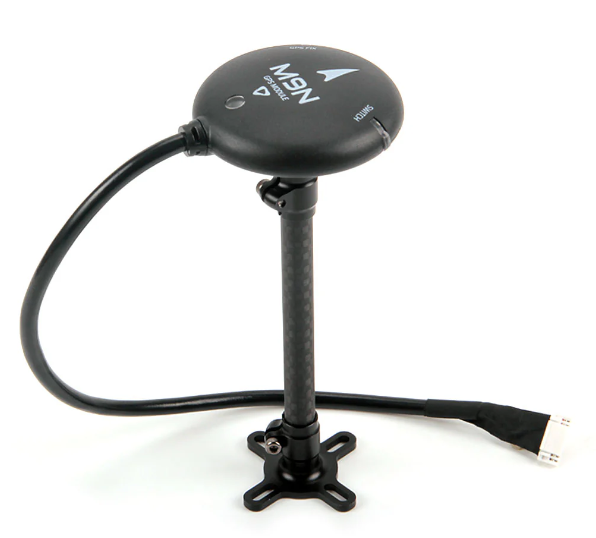
\includegraphics[width=.4\textwidth]{gps}
    \caption{GPS module for drones.}
    \label{fig:gps}
  \end{figure}
\end{frame}
\begin{frame}{The perception problem}{Tools for the job}
  \begin{figure}
    \centering
    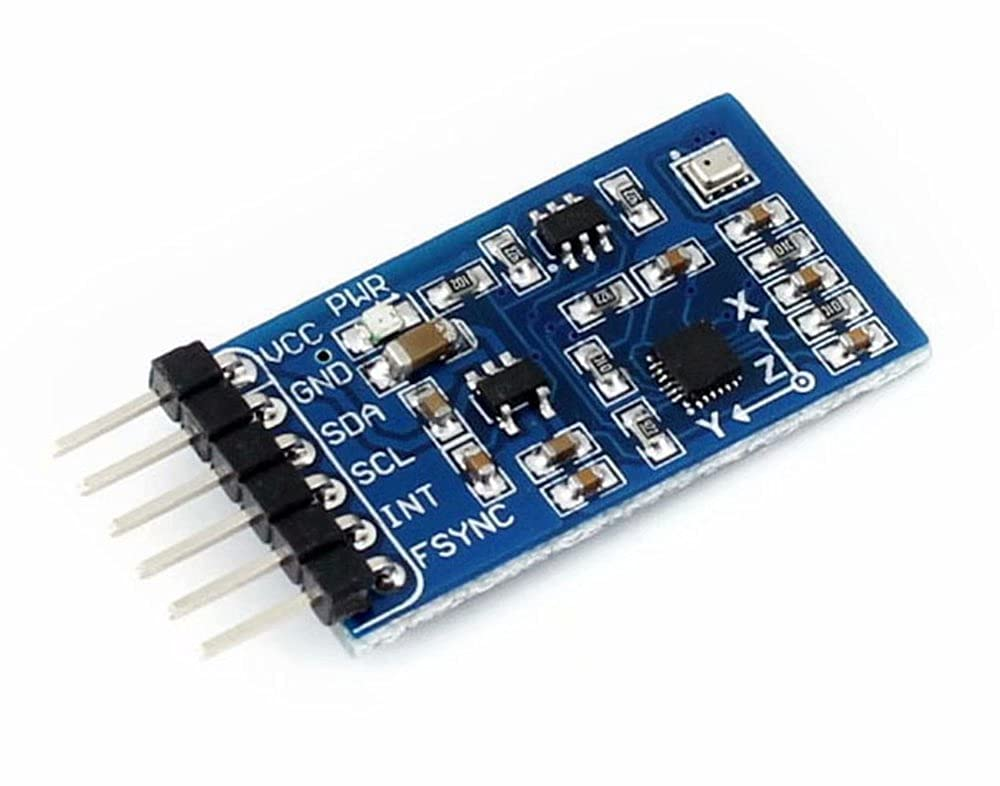
\includegraphics[width=.45\textwidth]{imu}
    \caption{Inertial Measurement Unit (IMU).}
    \label{fig:imu}
  \end{figure}
\end{frame}
\begin{frame}{The perception problem}{Tools for the job}
  \begin{figure}
    \centering
    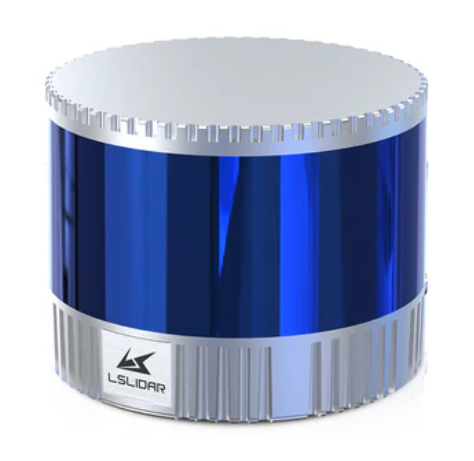
\includegraphics[width=.38\textwidth]{lidar}
    \caption{Light Detection and Ranging (LiDAR) sensor.}
    \label{fig:lidar}
  \end{figure}
\end{frame}
\begin{frame}{The perception problem}{Tools for the job}
  \begin{figure}
    \centering
    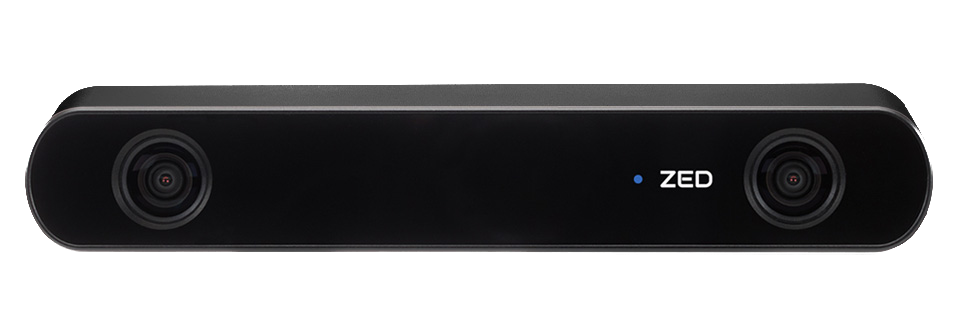
\includegraphics[width=.8\textwidth]{zed2i}
    \caption{ZED 2i stereo camera.}
    \label{fig:zed2i}
  \end{figure}
\end{frame}
